\section{Analysis}
\label{sec:Analysis}
To analyze the data collected in the LHCb experiment,
it is necessary to identify the $B_s$ events and distinguish them from the combinatorial background and other $B_0$ meson decays. 
As can be seen in \autoref{fig:Mass}, 
the mass distribution of the $B_s$ decay is not visible in the background. 
What is visible is the dominant $B_d$ decay.
\begin{figure}
    \centering
    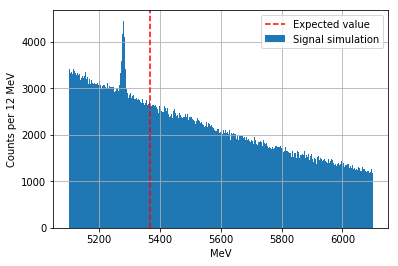
\includegraphics[width=0.8\textwidth]{bilder/Mass.png}
    \caption{Mass distribution of the LHCb Data.
        The $B_s$ decay is not visible in the background, while the dominant $B_d$ decay is visible.}
    \label{fig:Mass}
\end{figure}
To extract the $B_s$ sigal from the background, 
a Boosted Decision Tree (BDT) is used.
This BDT is trained on simulated data to distinguish between signal and background events.
To avoid overtraining,
the BDT is trained on a subset of features.
To find the optimal features a Multivariate Analysis (MVA) is performed.

\subsection{Multivariable Analysis}
\label{sec:MVA}
The BDT is trained using simulated signal events, 
while the background is taken directly from data. 
Background events are selected from the sideband of the invariant mass distribution, 
specifically from the region above the $B_s$ mass, 
where no signal contribution is expected. 
This approach avoids relying on simulated background, 
which is often less reliable than simulated signal.

Since the classifier is trained on a mixture of simulated (signal) and real (background) data, 
any systematic differences between simulation and data in a given feature has to be reduced.
To archieve this and ensure a reliable classifier, 
only features that are well described by the simulation are selected for BDT training. 
This agreement is quantified using a Kolmogorov-Smirnov test, 
and features exceeding a chosen threshold above $0.6$ are excluded from the training.

To use features that have a strong separation power between signal and background,
the separation power of each feature is calculated using the same Kolmogorov-Smirnov test.
Every feature with a distance below $0.5$ is also excluded from the training.

To prevent a training bias with respect to the invariant mass,
the correlation between the invariant mass and each feature is calculated.
Every feature with a correlation above $0.8$ is excluded from the training.
The remaining features and their correlation with the invariant mass are shown in \autoref{fig:Correlation}.
\begin{figure}
    \centering
    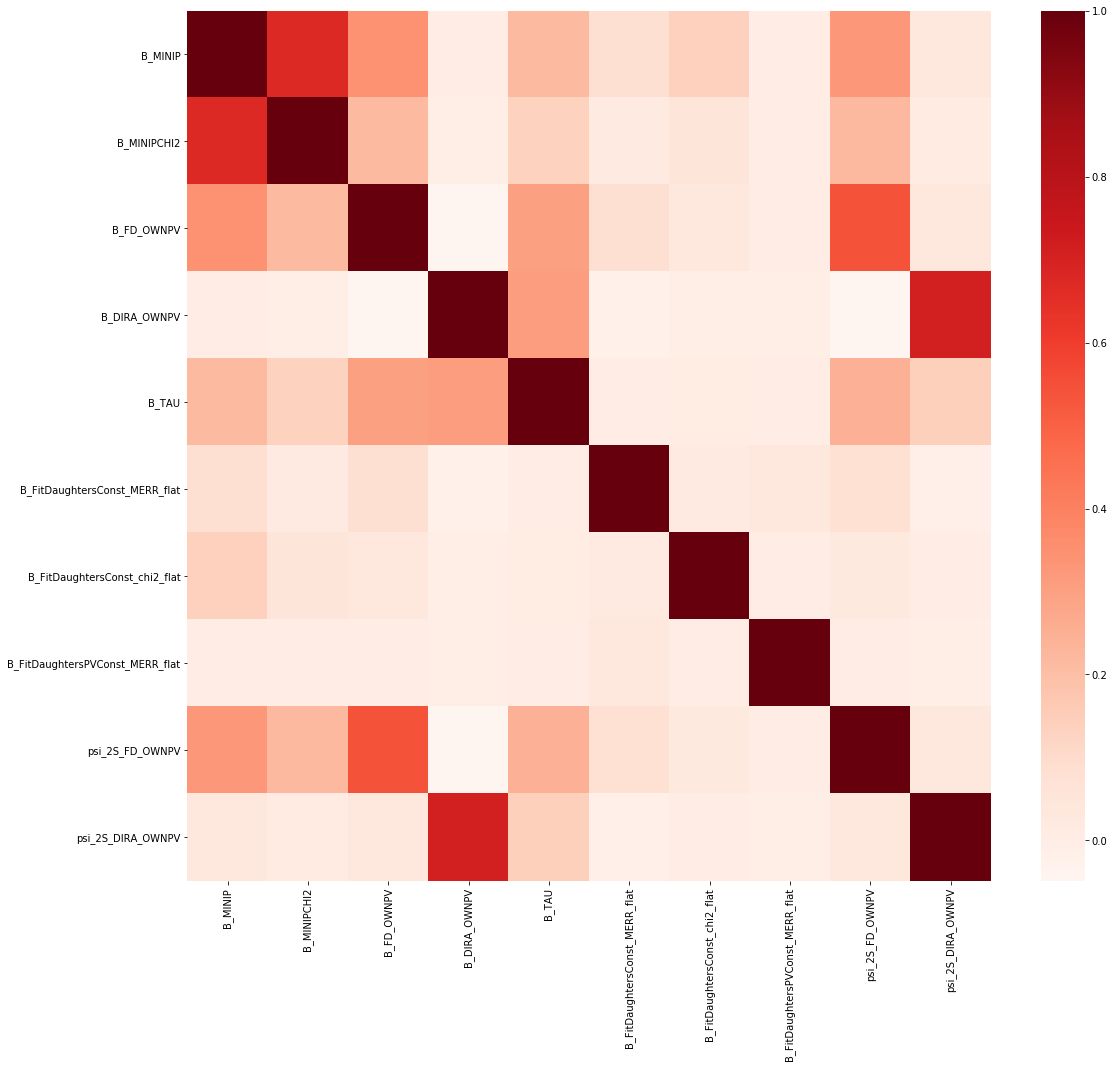
\includegraphics[width=0.5\textwidth]{bilder/Correlation.png}
    \caption{Correlation of the remaining features with the invariant mass.}
    \label{fig:Correlation}
\end{figure}    


\subsection{BDT}
\label{sec:BDT}
With the in \autoref{sec:MVA} selected features a BDT is trained to distinguish between signal and background events.
The BDT is trained on a subset of the data,
with the remaining data used for testing and validation.
This is repeated five times to different subsets of the data and traning events.
The BDT is trained using the \texttt{XGBoost} library.

The resulting distribution of the BDT output for the singal and background samples is shown in \autoref{fig:BDT},
which demonstrates the BDT's ability to effectively separate signal from background events.
\begin{figure}
    \centering
    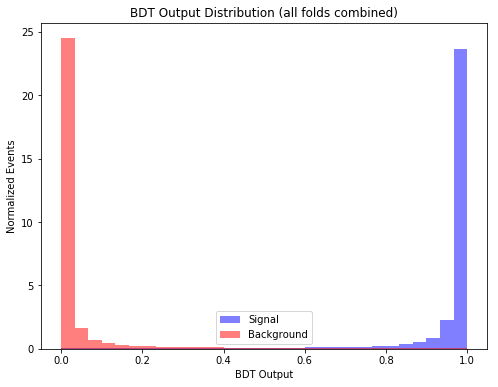
\includegraphics[width=0.5\textwidth]{bilder/BDT.png}
    \caption{Distribution of the BDT output for signal and background samples.}
    \label{fig:BDT}
\end{figure}

To evaluate the performance of the BDT, a Receiver Operating Characteristic (ROC) curve is generated and shown in \autoref{fig:ROC}.
The ROC curve illustrates the trade-off between the true positive rate (signal efficiency) and the false positive rate (background contamination) for different BDT output thresholds.
The area under the ROC curve (AUC) is calculated to quantify the overall performance of the BDT, with a value closer to 1 indicating better discrimination between signal and background.
\begin{figure}
    \centering
    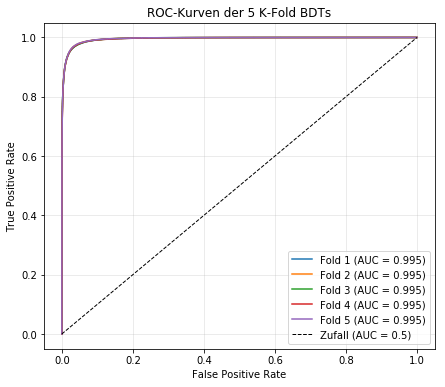
\includegraphics[width=0.5\textwidth]{bilder/ROC.png}
    \caption{Receiver Operating Characteristic (ROC) curve for the BDT.}
    \label{fig:ROC}
\end{figure}
A high AUC is archieved, indicating that the BDT is effective in distinguishing between signal and background events.
Also all five training iterations yield similar results, indicating that the BDT is stable.

To find the optimal BDT output threshold for event selection,
the significance of the signal is calculated for different thresholds.
As a figure of merit (FOM) for signal sensitivity, 
we use the Punzi significance,
\begin{equation}
    s = \frac{\epsilon_{\text{sig}}}{5/2 + \sqrt{n_{\text{bkg}}}},
\end{equation}
where $\epsilon_{\text{sig}}$ is the signal selection efficiency and $n_{\text{bkg}}$ is the number of background events in the signal region. 
The result is shown in \autoref{fig:FOM}, 
where the optimal BDT output threshold is determined to be $0.5$.
\begin{figure}
    \centering              
    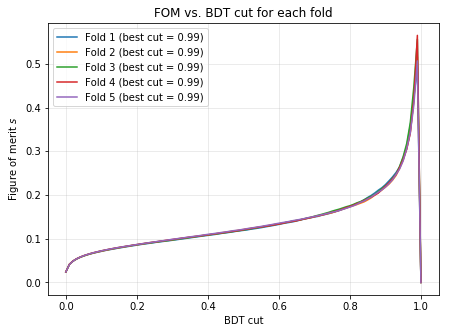
\includegraphics[width=0.5\textwidth]{bilder/FOM.png}
    \caption{Punzi significance as a function of the BDT output threshold.}
    \label{fig:FOM}
\end{figure}
The average best threshold of the five training iterations is at $0.99$.

\autoref{fig:BDT_Threshold} shows the effect of applying the BDT threshold to the data.
\begin{figure}
    \centering                      
    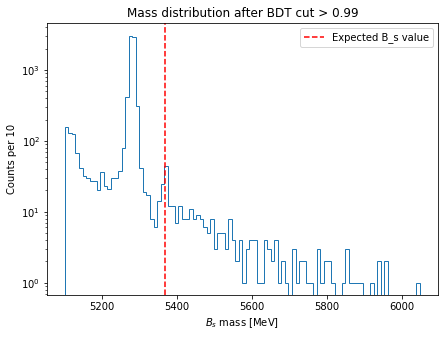
\includegraphics[width=0.5\textwidth]{bilder/BDT_Threshold.png}
    \caption{Distribution of the BDT output for signal and background samples after applying the optimal
    BDT output threshold.}
    \label{fig:BDT_Threshold}
\end{figure}
Two peaks can be seen in the region of the invariant mass for$B_s$ and $B_d$.


\subsection{Modeling the Mass Distribution}

To evaluate the trade-off between signal efficiency and background retention, 
the full invariant mass distribution needs to be modeled. 
The model consists of two peaking components, 
corresponding to the $B_d$ and $B_s$ signals, 
together with an exponential component describing the combinatorial background. 
To obtain a stable fit, 
the peak shapes are first determined by fitting the respective simulation samples, 
and the resulting shape parameters are subsequently fixed in the fit to data. 
The two signal fits are shown in \autoref{fig:Signal_Fits}.
\begin{figure}
    \centering
    \begin{subfigure}[b]{0.48\textwidth}
        \centering
        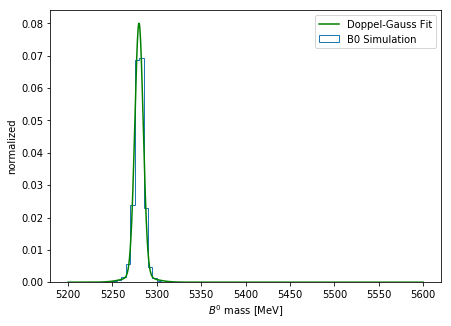
\includegraphics[width=\textwidth]{bilder/Signal_Fit_Bd.png}
        \caption{$B^0$ signal fit.}
        \label{fig:Signal_Fit_Bd}
    \end{subfigure}
    \hfill
    \begin{subfigure}[b]{0.48\textwidth}
        \centering
        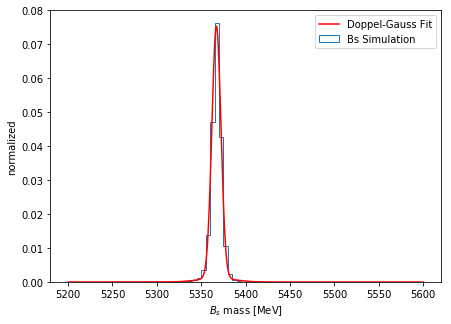
\includegraphics[width=\textwidth]{bilder/Signal_Fit_Bs.png}
        \caption{$B_s$ signal fit.}
        \label{fig:Signal_Fit_Bs}
    \end{subfigure}
    \caption{Fits to the simulated signal samples for $B^0$ (left) and 
    $B_s$ (right) decays, used to determine the peak shapes for the 
    subsequent fit to data.}
    \label{fig:Signal_Fits}
\end{figure}
Since the BDT selection can alter the peak shape, both 
simulated signal samples are classified and the BDT cut is applied 
before performing these fits, ensuring that the peak shapes obtained 
from simulation are representative of the shapes expected in data.

To account for the remaining combinatorial background, 
an additional component is included in the model, 
described by a decreasing exponential function.

The full mass distribution of the selected data is then fitted using this composite model, 
consisting of the two signal peaks, 
and the exponential background component.
\autoref{fig:Full_Fit} shows the resulting fit, 
together with its three submodels ($B^0$ signal, $B_s$ signal, and combinatorial background) overlaid on the selected data distribution.
\begin{figure}
    \centering
    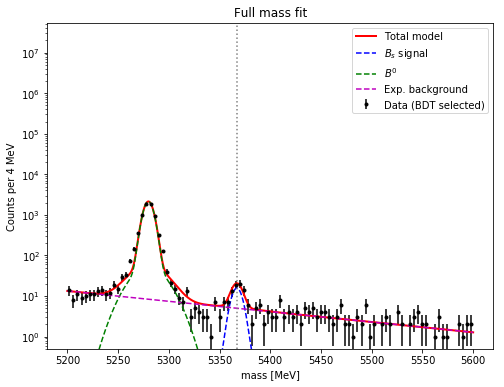
\includegraphics[width=0.7\textwidth]{bilder/Full_Fit.png}
    \caption{Fit to the full mass distribution of the selected data, 
    with fixed peak shapes for the $B^0$ and $B_s$ signal components 
    and a floating exponential background component. The individual 
    submodels are shown alongside the total fit and the selected data 
    distribution.}
    \label{fig:Full_Fit}
\end{figure}

We use a simple proxy for the significance, 
given by
\begin{equation}
    m = \frac{n_{\text{sig}}}{\sqrt{n_{\text{sig}} + n_{\text{bkg}}}},
\end{equation}
where $n_{\text{sig}}$ and $n_{\text{bkg}}$ denote the number of signal and background events, 
respectively, 
in the signal region.

The signal region is defined as $[5350.3, 5383.9]~\text{MeV}$, 
corresponding to an effective width of $\sigma_{\text{eff}} = 6.7~\text{MeV}$ around the $B_s$ peak. 
Integrating the fitted model over this region yields $n_{\text{sig}} = 50.8$ signal events and $n_{\text{bkg}} = 41.9$ background events. 
This results in a significance proxy of
\begin{equation}
    m = \frac{50.8}{\sqrt{50.8 + 41.9}} \approx 5.27.
\end{equation}